\documentclass{article}
\usepackage{settings}
\usepackage[normalem]{ulem}
%to write english paragraph \selectlanguage{language}
%to write english inline \textenglish{...}

\title{spring2023B}
\author{דורון שפיגל}
\date{08.04.24}

\begin{document}
\maketitle
\begin{Question}
נתון גביש דו מימדי מלבני עם וקטורי תא יחידה $\vec{a}=a\hat{x},\,\vec{b}=b\hat{y}\quad (b>a)$. הפוטנציאל הגבישי נתון על ידי הביטוי הבא:
$$U\left( x,y \right)=C_{0}\cos\left( \frac{2\pi}{a}x \right)\cos\left( \frac{2\pi}{b}y \right)+2C_{0}\cos\left( \frac{4\pi}{a}x \right)\cdot \cos\left( \frac{4\pi}{b}y \right)
$$
פער האנרגיה בנקודות הבאות מסומן באופן הבא:
$$\Delta E_{1}\left( k_{x}=\pi/a,\, k_{y}=0 \right),\, \Delta E_{1}\left( k_{x}=0,\, k_{y}=2\pi/b \right),\, \Delta E_{3}\left( k_{x}=0\, k_{y}=\pi/2b \right)$$
חשב: $\Delta E_{1},\, \Delta E_{2},\, \Delta E_{3}$.
\end{Question}
\begin{Answer}
פוטנציאל הגבישי נתון על ידי הביטוי הבא: $U\left( x,y \right)=\sum \limits^{}_{\vec{G}}{C_{G}e^{iG_{x}x+iG_{y}y}}$ כאשר $G$ הם וקטורים של השריג ההופכי. במקרה של תרגיל זה:
$$
G_{x}=\pm\frac{2\pi}{a}n,\, G_{y}=\pm\frac{2\pi}{b}n
$$ הביטוי שנתון בשאלה מורכב מסכום הכולל $n=$, האיבר הראשון, ו- $n=2$, האיבר השני.\\
פער האנרגיה נפתח עבור אותם $k$ שקרובים (או ממש נמצאים) בקצוות אזור ברילואן השונים. הפרש האנרגיה בקצה אזור ברילואן נתון על ידי הקשר הבא:
$$\Delta E\left( G/ 2 \right) = 2C_{G}$$
נמצא את המקדמים של $U(x,y)$ עבור הכיוונים השונים של התנע.
\begin{align*}
    U\left( x,0 \right)&=C_{0}\cos\left( \frac{2\pi}{a}x \right)+2C_{0}\cos\left( \frac{4\pi}{a}x \right)\\
    &=\frac{C_{0}}{2}\left( e^{i\frac{2\pi}{a}x}+e^{-i\frac{2\pi}{a}x} \right)+C_{0}\left( e^{i\frac{4\pi}{a}x}+e^{-i\frac{4\pi}{a}x} \right)\\
    U\left( 0,y \right)&=C_{0}\cos\left( \frac{2\pi}{b}y \right)+2C_{0}\cos\left( \frac{4\pi}{b}y \right)\\
    &=\frac{C_{0}}{2}\left( e^{i\frac{2\pi}{b}y}+e^{-i\frac{2\pi}{b}y} \right)+C_{0}\left( e^{i\frac{4\pi}{b}y}+e^{-i\frac{4\pi}{b}y} \right)
\end{align*}
עבור ההפרש הראשון:
\begin{align*}
    \Delta E_{1}\left( k_{x}=\pi/a,\, k_{y}=0 \right)&=\Delta E_{1}\left( k_{x}=\frac{1}{2}\frac{2\pi}{a},k_{y}=0\right)\\
    \Rightarrow &\Delta E_{1}\left( \frac{G=\frac{2\pi}{a}}{2} \right)=2C_{G=\frac{2\pi}{a}}=2\frac{C_{0}}{2}=C_{0}
\end{align*}
עבור ההפרש השני:
\begin{align*}
    \Delta E_{2}\left( k_{x}=0,\, k_{y}=2\pi/b \right)&=\Delta E_{2}\left( k_{x}=0,\, k_{y}=\frac{1}{2}\frac{4\pi}{b} \right)\\
    \Rightarrow &\Delta E_{2}\left( \frac{G=\frac{4\pi}{b}}{2} \right)=2C_{G=\frac{4\pi}{b}}=2C_{0}
\end{align*}
עבור ההפרש השלישי:
\begin{align*}
    \Delta E_{2}\left( k_{x}=0,\, k_{y}=\pi/2b \right)&=\Delta E_{2}\left( k_{x}=0,\, k_{y}=\frac{1}{2}\frac{\pi}{b} \right)\\
    \nexists n\in \mathbb{N}\quad \text{such that}\quad G_{x,y}=\frac{2\pi}{b}n=\frac{\pi}{b}\quad \Rightarrow &\Delta E_{3}\left( k_{x}=0,\, k_{y}=\pi/2b \right)=0
\end{align*}
ובסך הכל: ${\Delta E_{1}=C_{0}\neq0,\, \Delta E_{2}=2C_{0}\neq0,\, \Delta E_{3}=0}$.
\end{Answer}
\begin{Question}
מודל פשוט למעבר פאזה ממוצק לגז מבוסס על ההנחות הבאות: נתון שריג ריבועי דו מימדי עם $N$ אתרים המוצמד לאמבט חום בטמפרטורה $T$. בכל אתר נמצא אטום יחיד. כאשר האטום נמצא בפאזה המוצקה, האנרגיה של האתר היא שלילית: $\epsilon=-\epsilon_{0}$ כאשר $\epsilon_{0}>0$. כאשר האטום נמצא בפאזה הגזית, האנרגיה של האתר היא $\epsilon=0$. בנוסף, בפאזה הגזית הניוון של רמת האנרגיה היא $\Omega>>1$.\\
מה הביטוי למספר האטומים הנמצאים בפאזה המוצקה?
\end{Question}
\begin{Answer}
אחשב את פונקציית החלוקה,
הנוסחה לחישוב פונקציית החלוקה $Z$ היא:
\begin{align}\label{פונקציית החלוקה}
    1&=\sum \limits^{}_{S}{P\left( s \right)}=\frac{1}{Z}\sum \limits^{}_{S}{e^{-\beta E\left( s \right)}}\\
    \rightarrow&Z\triangleq \sum \limits^{}_{S}{g(s)e^{\frac{-E\left( s \right)}{kT} }}=\sum \limits^{}_{S}{g(s)e^{-\beta E\left( s \right)}}
\end{align}
ובמקרה שלנו:
\begin{align*}
    Z=1\cdot e^{\frac{-\left( -\epsilon_0 \right)}{kT}} + \Omega\cdot e^{\frac{-0}{kT}}=e^{\frac{\epsilon_0}{kT}}+\Omega
\end{align*}
ההסתברות להיות בפאזה המוצקה היא:
\begin{align*}
    P\left( s \right)=\frac{e^{-\beta E\left( s \right)}}{Z}=\frac{e^{\frac{\epsilon_0}{kT}}}{e^{\frac{\epsilon_0}{kT}}+\Omega}
\end{align*}
ולכן מספר האטומים בפאזה המוצקה יהיה מכפלת של מספר האטומים $N$ בסתברות להיות בפאזה המוצקה:
\begin{align*}
    n\left( \epsilon=-\epsilon_{0} \right)=N\cdot P\left( s \right)=N\cdot \frac{e^{\frac{\epsilon_0}{kT}}}{e^{\frac{\epsilon_0}{kT}}+\Omega}
\end{align*}
\end{Answer}
\begin{Question}
נתון מוצק תלת מימדי עם $N$ אתרים המוצמד לאמבט עם טמפרטורה $T$. בכל אתר נמצא אטום עם שתי רמות אנרגיה אפשריות. רמת יסוד עם $\epsilon_{g}=0$ ורמה מעוררת עם $\epsilon_{ex}=\epsilon_{0}$, מצא את הגרף המתאים לקיבול החום לאטום.
\end{Question}
\begin{Answer}
אחשב את פונקציית החלוקה:
\begin{align*}
    Z=1\cdot e^{\frac{-\epsilon_{g}}{kT}}+1\cdot e^{\frac{-\epsilon_{ex}}{kT}}=1+e^{\frac{-\epsilon_{0}}{kT}}
\end{align*}
כעת אחשב את האנרגיה הממוצעת במערכת, הנוסחה לחישוב האנרגיה הממוצעת על ידי פונקציית החלוקה היא:
\begin{align}\label{אנרגיה ממוצעת}
    \begin{cases}
        \langle E \rangle=\sum \limits^{}_{S}{E\left( s \right)P\left( s \right)}=\frac{1}{Z}\sum \limits^{}_{S}{E\left( s \right)e^{-\beta E\left( s \right)}}\\
        \pd{Z}{\beta}=\pd{}{\beta}\sum \limits^{}_{S}{e^{-\beta E\left( s \right)}}=-\sum \limits^{}_{S}{E\left( s \right)e^{-\beta E\left( s \right)}}
    \end{cases}\\
    \langle E \rangle=-\frac{1}{Z}\pd{Z}{\beta}\leftrightarrow\langle E \rangle=-\pd{}{\beta}\ln{Z}
\end{align}
ובמקרה שלנו:
\begin{align*}
    \langle E \rangle=-\pd{}{\frac{1}{kT}}\ln{\left( 1+e^{\frac{-\epsilon_{0}}{kT}} \right)}=-\frac{1}{1+e^{\frac{-\epsilon_{0}}{kT}}}\cdot \left( -\epsilon_{0}e^{\frac{-\epsilon_{0}}{kT}} \right)=\frac{\epsilon_{0}e^{\frac{-\epsilon_{0}}{kT}}}{1+e^{\frac{-\epsilon_{0}}{kT}}}
\end{align*}
כעת אחשב את הקיבול החום, הנוסחה לחישוב הקיבול החום היא:
\begin{align}\label{קיבול החום}
    C_{V}=\pd{\langle E \rangle}{T}
\end{align}
ולכן:
\begin{align*}
    \pd{}{T}\left( \epsilon_{0}e^{\frac{-\epsilon_{0}}{kT}} \right)&=\frac{\epsilon_{0}}{kT^{2}}\cdot\epsilon_{0}e^{\frac{-\epsilon_{0} }{kT}}=\frac{\epsilon_{0}^{2}}{kT^{2}}e^{\frac{-\epsilon_{0}}{kT}}\\
    num &= \frac{\epsilon_{0}^{2}}{kT^{2}}e^{\frac{-\epsilon_{0}}{kT}}\left( 1+e^{\frac{-\epsilon_{0}}{kT}} \right) - \frac{\epsilon_{0}^{2}}{kT^{2}}e^{\frac{-\epsilon_{0}}{kT}}\epsilon_{0}e^{\frac{-\epsilon_{0}}{kT}}\\
    &=\frac{\epsilon_{0}^{2}}{kT^{2}}e^{\frac{-\epsilon_{0}}{kT}}\\
    den &= \left( 1+e^{\frac{-\epsilon_{0}}{kT}} \right)^{2}\\
    C_{V}&=\frac{num}{den}=\frac{\frac{\epsilon_{0}^{2}}{kT^{2}}e^{\frac{-\epsilon_{0}}{kT}}}{\left( 1+e^{\frac{-\epsilon_{0}}{kT}} \right)^{2}}=\frac{\epsilon_{0}^{2}}{kT^{2}}\cdot\frac{e^{\frac{-\epsilon_{0}}{kT}}}{\left( 1+e^{\frac{-\epsilon_{0}}{kT}} \right)^{2}}
\end{align*}
כאשר $\epsilon_{0}>>kT \leftrightarrow T\to0$ הגורם $e^{\frac{-\epsilon_{0}}{kT}}$ מתנהג כמו $e^{-\infty}=0$ ולכן:
$$\limit{T\to0}{C_{V}}=\frac{\epsilon_{0}^{2}}{kT^{2}}\cdot\frac{0}{\left( 1+0 \right)^{2}}=0$$
כאשר $\epsilon_{0}<<kT \leftrightarrow T\to\infty$ היחס אז ישאף לאפס: ${\frac{\epsilon_{0}}{kT}}\to0$ ומקבלים ש:
$$\limit{T\to\infty}{C_{V}}=0\cdot\frac{\epsilon_{0}}{T}\cdot\frac{1}{\left( 1+1 \right)^{2}}=0$$
כלומר, על גרף הקיבול לשאוף לאפס עבור טמפרטורות נמוכות מאוד, ומאוד גבוהות.
\end{Answer}
\begin{Question}
נתונה צינורית פחמן חד מימדית מסוג מוליך למחצה עם יחס דיספריסה מהצורה הבאה:
$E\left( k_{x} \right)=\pm\sqrt{\Delta^{2}+\left( \hbar v_{0}k_{x} \right)^{2}}$ כאשר $v_{0}=10^{6}\left[ m/sec \right]$, $\Delta=0.4\left[ eV \right]$ (איור שמאלי). כתוצאה מאי סדר לאורך הצינורית זמן הפיזור הממוצע $\left( \tau \right)$ בטמפרטורות נמוכות מרמת פרמי מוצג באיור הימני. בנוסף נתון כי צפיפות נושאי המטען של האלקטרונים היא $n=6.35\cdot 10^{8}\left[ m^{-1} \right]$ ושהניוון של כל רמת אנרגיה הוא $4$ (שני ספינים ושני תתי שריגים). בהנחה שהטמפרטורה נמוכה מאוד יחסית לרמת פרמי, מהי רמת פרמי של צינורית הפחמן?\\
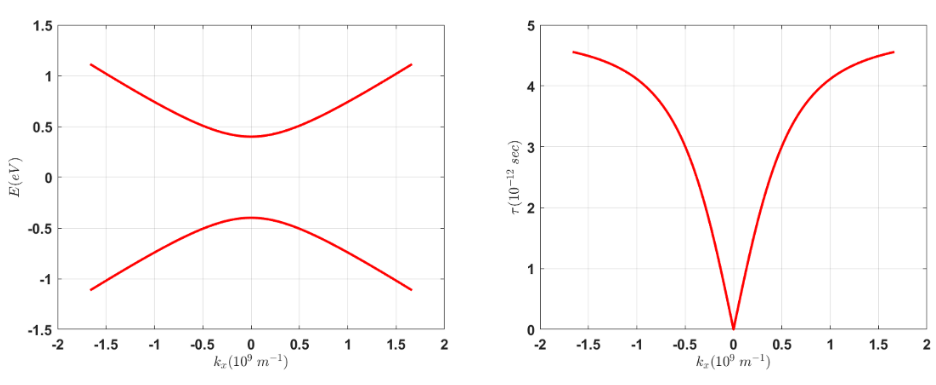
\includegraphics[width=0.9\textwidth]{image/Q4figure.png}
\end{Question}
\begin{Answer}
מספר המצבים עד מספר גל $k$ עבור מערכת באורך $L$ הוא:
\begin{align}\label{מספר מצבים}
    N\left( k \right)&=2\cdot\frac{k}{\frac{\pi}{L}}\tag{1d}\\
    N\left( k \right)&=2\cdot\frac{\pi k^{2}}{4\left( \frac{\pi^2}{L^{2}} \right)}\tag{2d}\\
    N\left( k \right)&=2\cdot\frac{\frac{1}{8}\cdot\frac{4\pi}{3}k^{3}}{\left( \frac{\pi}{L} \right)^{3}}\tag{3d}
\end{align}
ובמקרה אצלנו, צינורית פחמן חד מימדית, נקבל:
$$N\left( k \right)=2\cdot\frac{k}{\frac{\pi}{L}}$$
מספר מצבים ליחידת $V$ הוא:
\begin{align}
    n\left( \epsilon \right)=\text{ degenerate}\cdot \frac{N\left( k \right)}{V}
\end{align}
ובמקרה אצלנו:
\begin{align*}
    \begin{cases}
        V=2L&\text{כי יש שני תת שריגים}\\
        \text{degenerate}=4&\text{ניוון רמת אנרגיה}
    \end{cases}
\end{align*}
ומקבלים:
\begin{align*}
    n&=4\cdot \frac{2\cdot\frac{k_{f}}{\frac{\pi}{L}}}{2L}=4\cdot \frac{k_{f}}{\pi}\\
    \longrightarrow& k_{f}=\frac{\pi n}{4}=6.35\cdot \frac{\pi}{4}\cdot 10^{8}=0.498\cdot 10^{9}\left[ m^{-1} \right]
\end{align*}
כעת לפי הגרף השמאלי, רמת פרמי צריכה להימצא בין הפסים, ולכן עבור $k_{f}\approx0.5\cdot10^{9}$ נקבל ש $E_{f}=0.5\left[ eV \right]$.
\end{Answer}
\begin{Question}
מהו מרחק הפיזור הממוצע ${\left( l_{mfp} \right)}$ בטמפרטורות נמוכות יחסית לרמת פרמי של צינורית הפחמן המתוארת בשאלה הקודמת?
\end{Question}
\begin{Answer}
מרחק הפיזור הממוצע הוא:
\begin{align}\label{מרחק פיזור ממוצע}
    l_{mfp}=v_{f}\cdot\tau
\end{align}
את זמן הפיזור הממוצע אמצע לפי הגרף הימני בשאלה הקודמת עבור $k_{f}=0.5\cdot10^{9}\left[ m^{-1} \right]$ נקבל ש:
$$\tau=3\cdot10^{-12}\left[ sec \right]$$
מהירות פרמי נתונה לפי:
$$v_{f}=\frac{P_{f}}{m_{0}}=\frac{1}{\hbar}\pd{E_{k}}{k}$$
אחשב את הנגזרת:
\begin{align*}
    \pd{E_{k}}{k}&=\pd{\sqrt{\Delta^{2}+\left( \hbar v_{0}k_{x} \right)^{2}}}{k}=
    \frac{1}{2}\frac{1}{\sqrt{\Delta^{2}+\left( \hbar v_{0}k_{x} \right)^{2}}}\cdot2\left( \left( \hbar v_{0} \right)^{2}k_{x} \right)\\
    &=\frac{\left( \hbar v_{0} \right)^{2}k_{x}}{\sqrt{\Delta^{2}+\left( \hbar v_{0}k_{x} \right)^{2}}}=
    \frac{\left( \hbar v_{0} \right)^{2}k_{x}}{E\left( k_{x} \right)}
\end{align*}
ולכן:
\begin{align*}
    v_{f}&=\frac{1}{\hbar}\pd{E_{k}}{k}=
    \frac{ \hbar\left( v_{0} \right)^{2}k_{x}}{E\left( k_{x} \right)}=\frac{1.05\cdot10^{-34}\cdot\left( 10^{6} \right)^{2}\cdot0.5\cdot10^{6}}{0.5\cdot1.6\cdot10^{-19}}\\&=0.65625\cdot10^{6}\left[ m/sec \right]\\
    \Rightarrow& l_{mph}=v_{f}\cdot\tau=0.65625\cdot10^{6}\cdot 3\cdot10^{-12} = 1.96875 \cdot 10^{-6}=1.95\left[ \mu m \right]
\end{align*}
\end{Answer}
\begin{Question}
נתונות 2 מערכות דו ממדיות עם שטח זהה $A$. יחסי הנפיצה של האלקטרונים במערכת הראשונה והשנייה נתונים על ידי הביטויים הבאים בהתאמה:
\begin{align*}
    \epsilon_{1}\left( \vec{k} \right)&=\frac{\hbar^{2}}{2m}k_{x}^{2}+\frac{\hbar^{2}}{2m}k_{y}^{2}\\
    \epsilon_{2}\left( \vec{k} \right)&=\hbar c\abs{\vec{k}}^{\frac{1}{a}}\\
    &&0<a,c\in\Re
\end{align*}צפיפות המצבים ליחידת שטח עבור כל מהמערכות:\\
עבור המערכת הראשונה, ראינו בתרגול כי:
$$g_{1}\left( \epsilon \right)=\frac{m}{\pi\hbar^{2}}$$
עבור המערכת השנייה:\\
נתון כי השטח הוא $A$, כלומר, עבור קופסה דו ממדית עם צלעות $L$ נקבל: $A=L^{2}$. מצבי התנע המותרים הם $k_{x}=\frac{\pi n_{x}}{L},\, k_{y}=\frac{\pi n_{y}}{L}\quad n=1,2,3,\dots$ ולכן, המרחק בין כל 2 נקודות תנע הוא $\frac{\pi}{L}$, אפשר לחלק את מערכת הצירים לריבועים באורכים $\frac{\pi}{L}\times\frac{\pi}{L}$ ואז שטח של מצב בודד הוא:
$$V_{single-state}=\left( \frac{\pi}{L} \right)^{2}=\frac{\pi^{2}}{A}$$
נסתכל על רדיוס עקום שווה אנרגיה:
\begin{align*}
    \epsilon_{2}&=\hbar c\abs{\vec{k}}^{\frac{1}{a}}\\
    \abs{\vec{k}}&=\left( \frac{\epsilon_{2}}{\hbar c} \right)^{a}\\
    0<a,c,\epsilon\in\Re&\implies 0<\left( \frac{\epsilon_{2}}{\hbar c} \right)^{a}\in\Re\\
    &\implies \abs{\vec{k}}=\vec{k}=\left( \frac{\epsilon_{2}}{\hbar c} \right)^{a}
\end{align*}
$\sum\left( \epsilon \right)$ הוא שטח מעגל בעל רדיוס $\left( \frac{\epsilon_{2}}{\hbar c} \right)^{a}$, ולכן:
\begin{align*}
    \sum\left( \epsilon \right)=\pi\cdot\text{radius}^{2}=\pi\left( \frac{\epsilon_{2}}{\hbar c} \right)^{2a}
\end{align*}
ולפי
נוסחה לצפיפות מצבים:
\begin{equation}
    g\left( \epsilon \right)=\frac{d}{d\epsilon}\underbracket[0.1ex]{\left[ 
        \text{\footnotesize{\#degenerate}}\cdot\sum\left( \epsilon \right)\cdot \frac{1}{V_{single-state}\cdot \text{\footnotesize{\#sub-lattice}}}
        \cdot \underbracket[0.1ex]{2}_{\text{spin}}\cdot \frac{1}{2^{\left\{ d:0,2,3 \right\}}}\cdot
        \frac{1}{V_{system}}
    \right]}_{=n}
\end{equation}
ולכן:
\begin{align*}
    g\left( \epsilon_{2} \right)&=\frac{d}{d\epsilon}\left[ 1
    \cdot  \pi\left( \frac{\epsilon_{2}}{\hbar c} \right)^{2a}
    \cdot \frac{1}
    {\frac{\pi^{2}}{A}\cdot1}
    \cdot2
    \cdot\frac{1}{2^{2}}
    \cdot\frac{1}{A}
    \right]\\
    g\left( \epsilon_{2} \right)&=\frac{d}{d\epsilon}\left[
    \cancel{\pi}\left( \frac{\epsilon_{2}}{\hbar c} \right)^{2a}
    \cdot \frac{\cancel{A}}
    {\pi^{\cancel{2}}}
    \cdot\cancel{2}
    \cdot\frac{1}{2^{\cancel{2}}}
    \cdot\frac{1}{\cancel{A}}
    \right]
    =\frac{d}{d\epsilon}\left[ 
        \left( \frac{\epsilon_{2}}{\hbar c} \right)^{2a}\cdot\frac{1}{2\pi}
    \right]\\
    g_{2}\left( \epsilon \right)&=\frac{\cancel{2}a\cdot \epsilon^{2a-1}}{\left( \hbar c \right)^{2}}\cdot\frac{1}{\cancel{2}\pi}=\boxed{\frac{a\cdot \epsilon^{2a-1}}{\pi\left( \hbar c \right)^{2a}}}\\
\end{align*}
כעת, נתון כי שומרים על טמפרטורה השואפת לאפס בשתי המערכות.\\
נתון שמספר האלקטרונים בשתי המערכות הוא $N$, מחברים את שתי המערכות באמצעות תיל מוליך. אחרי זמן ארוך מאוד, מודדים את צפיפות האלקטרונים בשתי המערכות ומוצאים שהצפיפויות שוות. מהו $c$?\\
זמן ארוך מאוד $\Leftrightarrow$ שיווי משקל, המערכות מחוברות בתיל ולכן מחליפות חלקיקים, כלומר יש שוויון פוטנציאל כימי: $\mu_{c1}=\mu_{c2}$. ידוע כי בטמפרטורות נמוכות $E_{f}\triangleq \mu_{c}\left( T=0 \right)$, אזי, יש שוויון בין אנרגיות פרמי של המערכות.
\begin{align*}
    g_{1}\left( \epsilon \right)=\frac{m}{\pi\hbar^{2}}\rightarrow n_{f}&=\int_{0}^{\epsilon_{f1}}{g_{1}\left( \epsilon \right)d\epsilon}=\frac{m\epsilon_{f1}}{\pi\hbar^{2}}\\
    %solve((m*e)/(pi*h**2)-n, e)[0] = pi*h**2*n/m
    \Rightarrow \epsilon_{f1}&=\frac{\pi\cdot\hbar^{2}\cdot n}{m}\\
    g_{2}\left( \epsilon \right)=\frac{a\cdot \epsilon^{2a-1}}{\pi\left( \hbar c \right)^{2a}}
    \rightarrow n_{f}&=\int_{0}^{\epsilon_{f2}}{g_{2}\left( \epsilon \right)d\epsilon}=
    \left( \frac{\epsilon_{2}}{\hbar c} \right)^{2a}\cdot\frac{1}{2\pi}\\
    \Rightarrow \epsilon_{f2}&=\left( 2\pi\cdot n \right)^{\frac{1}{2a}}\cdot\hbar c
\end{align*}
מהנתון שצפיפויות האלקטרונים שוות, ומזה שבסך הכל בשתי המערכות יחדיו יש $N$ אלקטרונים, אז הצפיפות בכל מערכת היא: $n=\frac{N}{2}\cdot\frac{1}{A}$.
אציב את $n$ בכל רמת פרמי ואשווה:
\begin{align*}
    \epsilon_{f1}&=\frac{\pi\cdot \hbar^{2}\cdot n}{m} = \frac{\pi N \hbar^{2}}{2 A m}\\
    \epsilon_{f2}&=\left( 2\pi\cdot n \right)^{\frac{1}{2a}}\cdot\hbar c=c \hbar \left(\frac{\pi N}{A}\right)^{\frac{1}{2 a}}\\
    %\left( 2\pi\cdot n \right)^{\frac{1}{2a}}\cdot h c = c \hbar (\frac{\pi N}{A})^{\frac{1}{2 a}}
    \epsilon_{f1}=\epsilon_{f2}\rightarrow c&=\frac{\pi N \hbar (\frac{\pi N}{A})^{- \frac{1}{2 a}}}{2 A m}
\end{align*}
מהו התנע הגדול ביותר של האלקטרונים בכל אחת מהמערכות?\\
מספר המצבים עד מספר גל $k$ עבור מערכת באורך $L$ הוא:
\begin{align*}
    N\left( k \right)&=2\cdot\frac{k}{\frac{\pi}{L}}\tag{1d}\\
    N\left( k \right)&=2\cdot\frac{\pi k^{2}}{4\left( \frac{\pi^2}{L^{2}} \right)}\tag{2d}\\
    N\left( k \right)&=2\cdot\frac{\frac{1}{8}\cdot\frac{4\pi}{3}k^{3}}{\left( \frac{\pi}{L} \right)^{3}}\tag{3d}
\end{align*}
במקרה פה, המערכת היא מ 2 מימדים, ולכן:
$$N\left( k \right)=\frac{A k^{2}}{2\pi}$$
אחשב תנע פרמי עבור מערכת 1:
\begin{align*}
    \begin{cases}
        \epsilon_{1}=\frac{\hbar^{2}\cdot k^{2}}{2m}&\text{יחס נפיצה נתון}\\
        \epsilon_{f1}=\frac{\pi\cdot N\cdot\hbar^{2}}{2\cdot A\cdot m}&\text{רמת פרמי}
    \end{cases}\rightarrow k_{f}=\sqrt{\frac{\pi\cdot N}{A}}
\end{align*}
אחשב תנע פרמי עבור מערכת 2:
\begin{align*}
    \begin{cases}
        \epsilon_{{2}}=\hbar c\cdot k^{\frac{1}{a}}&\text{יחס נפיצה נתון}\\
        \epsilon_{{f2}}=c\cdot\hbar\left( \frac{\pi N}{A} \right)^{\frac{1}{2a}}&\text{רמת פרמי}
    \end{cases}\rightarrow k_{f}=\sqrt{\frac{\pi\cdot N}{A}}
\end{align*}
כעת מסירים את התייל שמחבר את שתי המערכות ולאחר מכן מוסיפים אלקטרונים למערכת 2, כך שנוצר מתח חשמלי בין המערכות.\\ כיצד אנרגיית פרמי משתנה במערכת 2 (גדלה/ קטנה) והאם היא משתנה במערכת 1?\\
ראינו כי אנרגיית פרמי בכל מערכת תלויה במספר האלקטרונים שבה,לכן הוספת אלקטרונים למערכת 2 תגדיל בה את רמת פרמי, לא הוספנו או החסרנו אלקטרונים ממערכת 1 ולכן רמת פרמי בה לא משתנה.\\
כעת, מחברים את שתי המערכות באמצעות תיל מוליך. נתייחס לתיל כאל מערכת תלת מימדית של גליל שהציר הראשי שלו (ציר $x$) ארוך מאוד, והוא מחבר את שתי המערכות.\\ יחס הנפיצה של האלקטרונים בתיל נתונה על ידי הביטוי הבא:
\begin{align*}
    \epsilon\left( \vec{k} \right)=\frac{\hbar^{2}}{2m_{x}}k_{x}^{2}+\frac{\hbar^{2}}{2m_{y}}k_{y}^{2}+\frac{\hbar^{2}}{2m_{z}}k_{z}^{2}
\end{align*}
צפיפות האלקטרונים בתייל היא $n_{0}$ וזמן הפיזור הממוצע הוא $\tau_{0}$. רשמו ביטוי למוליכות החשמלית שנמדדה בתיל.\\
מוליכות החשמלית היא: $\sigma=\frac{1}{\rho}=\frac{nq^{2}\tau}{m}$, נתון אצלנו:
$$\begin{cases}
    n=n_{0}&\text{צפיפות אלקטרונים בתיל}\\
    q=-e&\text{אלקטרונים}\\
    \tau=\tau_{0}&\text{זמן פיזור ממוצע}
\end{cases}
$$
המסה $m$ בנוסחה היא המסה האפקטיבית, 
\begin{align*}
    \frac{1}{m}&=\begin{pmatrix}
        \frac{1}{m_{x}}&0&0\\
        0&\frac{1}{m_{y}}&0\\
        0&0&\frac{1}{m_{z}}
    \end{pmatrix}
\end{align*}
ואקבל את טנזור המוליכות החשמלית:
$$\sigma = n_{0}\cdot e^{2}\cdot\tau_{0}\begin{pmatrix}
    \frac{1}{m_{x}}&0&0\\
    0&\frac{1}{m_{y}}&0\\
    0&0&\frac{1}{m_{z}}
\end{pmatrix}
$$
לפי חוק אום, צפיפות זרם היא המכפלה בין המוליכות לשדה החשמלי, במקרה פה, השדה הוא בכיוון המחבר את שתי המערכות: $E=E\hat{x}$, ולכן:
$$\vec{J}=\sigma\vec{E}=n_{0}\cdot e^{2}\cdot\tau_{0}
\begin{pmatrix}
    \frac{1}{m_{x}}&0&0\\
    0&\frac{1}{m_{y}}&0\\
    0&0&\frac{1}{m_{z}}
\end{pmatrix}\cdot
\begin{pmatrix}
    \hat{x}\\
    0\\
    0
\end{pmatrix} = n_{0} \tau_{0} e^{2} \begin{bmatrix}\frac{E}{m_{x}}\\0\\0\end{bmatrix}=\frac{n_{0} \tau_{0} e^{2}E}{m_{x}}\hat{x}
$$
ורכיב המוליכות בכיוון $\hat{x}$ בצפיפות הזרם הוא:
$$\sigma_{xx}=\frac{J_{x}}{E}=\frac{n_{0} \tau_{0} e^{2}}{m_{x}}$$
\end{Question}
\begin{Question}
נתון הגביש הבא:\\
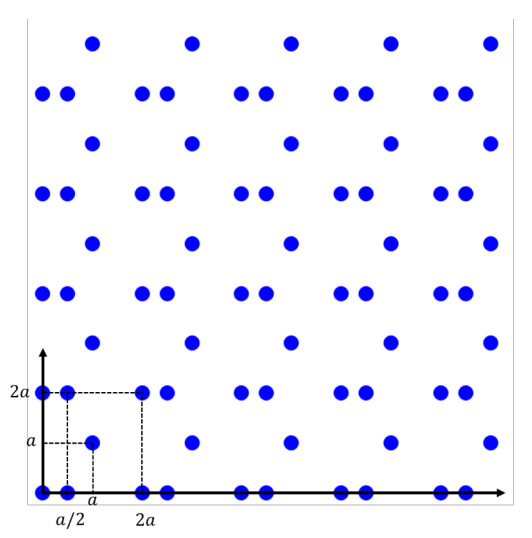
\includegraphics[width=0.9\textwidth]{image/Q71.png}\\
הווקטורים הראשוניים של הגביש הם:
$$\begin{cases}
    a_{1}=2a\hat{x}\\
    a_{2}=2a\hat{y}
\end{cases}
$$
ווקטורי הבסיס הם:
$$\begin{cases}
    d_{1}=0\\
    d_{2}=\frac{a}{2}\hat{x}\\
    d_{3}=a\hat{x}+a\hat{y}
\end{cases}
$$ כמתואר בציור:\\
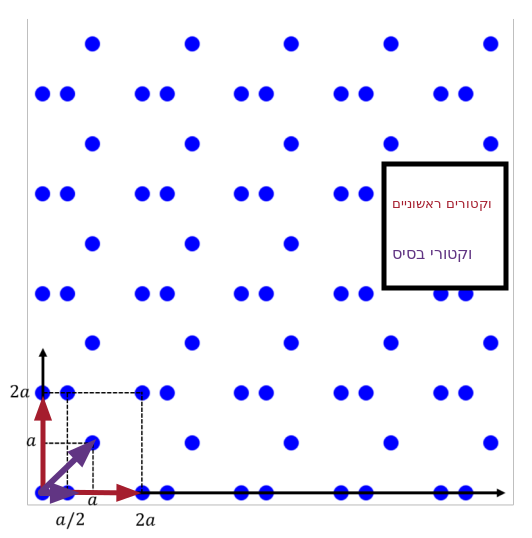
\includegraphics[]{image/Q72.png}\\
תא Wigner-Seitz של הגביש הוא תא ריבועי:\\
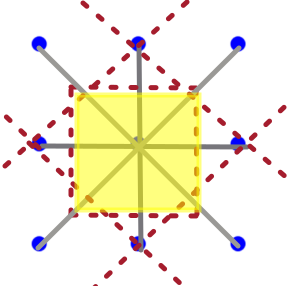
\includegraphics[]{image/Q73.png}\\
כדי למצוא את הווקטורים של השריג ההופכי, תחילה אחשב את שטח תא היחידה הנפרש על ידי הוקטורים הראשוניים:
$$S=\abs{\vec{a_{1}}\times \vec{a_{2}}}=\abs{2a\hat{x}\times 2a\hat{y}}=4a^{2}
$$
כעת, אמצע את הווקטורים הראשונים של הסריג ההפכי:
$$\begin{cases}
    \vec{b_{1}}=2\pi\frac{\vec{a_{2}}\times\hat{z}}{S}=\frac{\pi}{2a^{2}}\cdot2a\hat{y}\times\hat{z}=\frac{\pi}{a}\hat{x}\\
    \vec{b_{2}}=2\pi\frac{\hat{z}\times\vec{a_{1}}}{S}=\frac{\pi}{2a^{2}}\cdot2a\hat{z}\times\hat{x}=\frac{\pi}{a}\hat{y}
\end{cases}
$$
השריג ההפכי הוא ריבוע עם אורך צלע $\frac{\pi}{a}$.\\
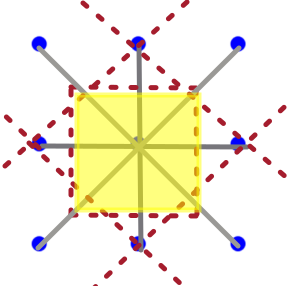
\includegraphics[]{image/Q73.png}\\
מבלי לפתור את הבעיה, ניתן לראות שווקטור הבסיס של תא היחידה הולך ל 3 אטומים, לכל אטום אורביטל אחד, לכן נצפה לקבל שלושה פסי אנרגיה.\\
\sout{
נתון כעת הגביש הבא:\\
%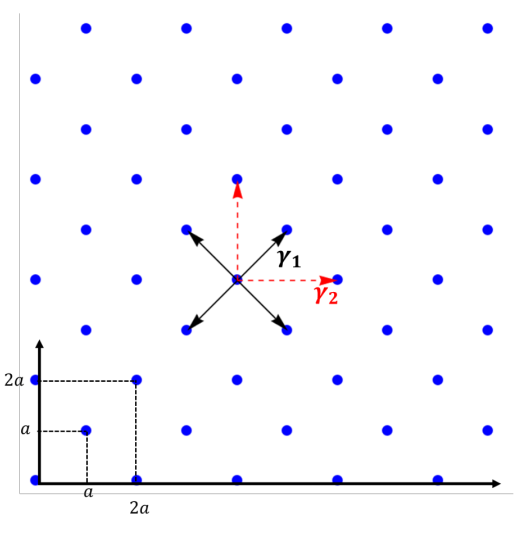
\includegraphics[]{image/Q74.png}\\
נניח שהצימוד בין השכנים הוא $\gamma_{1}=\gamma,\, \gamma_{2}=0$ והאנרגיה של האורביטלים הינה $E_{0}$. נתייחס רק לשכנים עם הצימוד $\gamma_{1}$ ונמצא את מבנה הפסים בעזרת שיטת הקשירה ההדוקה.\\}


\end{Question}








\end{document}